\documentclass[11pt]{article}

\usepackage[a4paper,margin=2.5cm]{geometry}
\usepackage{amsmath,amssymb}
\usepackage{microtype}
\usepackage[T1]{fontenc}
\usepackage{parskip}
\usepackage{graphicx}
\usepackage{tikz}
\usetikzlibrary{arrows.meta}
\definecolor{loopone}{HTML}{2C5F8A}
\definecolor{looptwo}{HTML}{2E7D6B}
\definecolor{loopthree}{HTML}{B5852F}
\definecolor{edgc}{HTML}{343A40}
\definecolor{anc}{HTML}{AEB4BA}

\newcommand{\code}[1]{\texttt{#1}}

\title{
Knowledge-First Forward Modelling:\\
Discovering Mechanisms and Measurements before Estimating Parameters\\[4pt]
\large Salivary gland branching morphogenesis as a case study in Plexus
}
\author{}
\date{}

\begin{document}
\maketitle

\begin{abstract}
Modern differentiable simulators have transformed parameter estimation. Once a forward model has been specified, gradients efficiently recover parameter values that reproduce experimental observations. They do not answer a more fundamental question: \emph{what should the forward model be?} In developmental biology this question is often the limiting one. Numerous mechanisms have been proposed---reaction--diffusion, differential adhesion, collective migration, extracellular-matrix guidance, mechanical buckling---yet it remains unclear which combinations are sufficient to reproduce the observed morphogenesis.

Our thesis is one sentence: \textbf{parameter estimation, forward-model discovery, and measurement discovery are three distinct scientific inference problems; they should not be solved by the same optimization loop.} Plexus provides the language on which the three operate---biological systems expressed as compositions of reusable operators acting on sets, states, fields and maps. The first problem is a search over operator \emph{compositions}: rather than fit one predetermined simulator, explore which compositions generate the phenotype and characterize the morphology manifold they span. The second is differentiable inverse modelling: once a composition is fixed, its operators expose gradients and descent recovers the parameters that reproduce a specimen---the regime of our companion cardiomyocyte study. The third is measurement discovery: a simulation is compared to data only through a metric, metrics are themselves hypotheses, and the descriptor that certifies one morphology as a match can dismiss another---so the metric must be discovered, not assumed.

We couple the three as loops that communicate through a single immutable object, the \emph{RunRecord}: every simulation becomes a record, and knowledge is \emph{distilled} from records rather than read off a simulation. Using embryonic salivary gland branching as a case study, we show the loops climbing a bootstrap ladder---a trusted coarse metric, a first robust mechanism, and, when that metric proves too coarse to separate rival mechanisms, a first improved measurement that reopens the mechanism conclusion---while a differentiable fit, verified here on a synthetic recoverable case, is earned last. The loops are designed to reinforce one another: better mechanisms enable better fits, fits expose structured residuals, and residuals and degeneracies motivate better measurements and new operators.

The result is not a single best simulation but a progressively refined language for branching morphogenesis. Published models become particular compositions within this language rather than competing frameworks, allowing mechanisms to be compared, combined, and ultimately rediscovered from data instead of selected a priori.
\end{abstract}

\section*{A joint problem: which model, which parameters, which metric}

Parameter optimization presupposes a model. Given a plausible forward model, gradients estimate its parameters efficiently---the situation once the model is trusted. But in development the model itself is the unknown, and estimating parameters before discovering the mechanism only finds a compensating artifact that fits the data without capturing how the system works. Worse, the three questions are not separable: the best-fitting parameters depend on the model, and whether a model \emph{looks} right depends on the metric. Fixing the model and the metric and optimizing only the parameters is safe just when both are already correct.

Plexus makes the model a searchable object. It expresses a biological system as a composition of reusable \emph{operators} acting on \emph{sets} (agents, particles, cells), \emph{states}, \emph{fields} (grids), and \emph{maps} (how one couples to another); a forward model is therefore not a monolithic program but a \emph{spec}---which operators are present and how they are wired. Freely composed, these primitives span a space far larger than any hand-built model---one that \emph{contains} the published mechanisms as special cases but also every untested mixture and compositions no one has written down. This matters because the mechanisms in the literature are almost always studied one at a time; their mixtures are rarely tested, yet a mixture is the likeliest explanation of a phenotype that no single mechanism fully reproduces. Forward-model discovery becomes a well-posed search over compositions, in which a Turing model and an adhesion model are not rival codebases but two points in one composition space, to be compared on equal footing, combined, and---the goal---rediscovered from data rather than selected a priori.

The scientific state is therefore the triple $(C,\theta,\phi)$: a composition $C$, its parameters $\theta$, and the descriptor $\phi$ that measures agreement with data. The rest of this paper is about inferring the three without conflating them.

\section*{The RunRecord: simulation, not knowledge}

A single rule organizes the whole system:
\[
\text{simulation}\ \longrightarrow\ \text{RunRecord}\ \longrightarrow\ \text{knowledge}
\qquad(\text{never } \text{simulation}\longrightarrow\text{knowledge}).
\]
A \emph{RunRecord} is the immutable, reproducible evidence of one simulation: the composition $C$, parameters $\theta$, seed, backend, and the resulting morphology. Two guardrails make it trustworthy. First, its raw facts are frozen after creation; a new metric never rewrites them but is \emph{appended} as a versioned analysis (\,$\text{analyses}[\phi_1]$, $\text{analyses}[\phi_2],\dots$), so raw evidence survives every change of measurement. Second, composition identity---a structural hash of the operator graph, excluding parameter values---is kept separate from run identity, which also fixes $\theta$, seed and backend; the same composition can have many runs. The archive of RunRecords is the source of truth. \emph{Knowledge} is a separate, distilled interpretation that is revised as evidence accumulates, and it sorts every claim into four classes: \textbf{Established} (a mechanism that is necessary, sufficient, and robust), \textbf{Refuted} (a hypothesis contradicted across seeds), \textbf{Structural limitation} (a composition that \emph{cannot} produce the phenotype---``adhesion alone cannot branch,'' stronger than ``false'' and reusable), and \textbf{Open}. A mechanism claim is promoted only when it answers, as a biology paper would, three questions: is the operator \emph{necessary} (ablate it---does the phenotype collapse?), \emph{sufficient} (does a minimal composition containing it emerge?), and \emph{robust} (across seeds and a parameter basin)?

\section*{A precondition: the substrate must be able to express the phenotype}

Before any composition of operators can generate the phenotype, the \emph{substrate}---the state representation the operators act on, i.e.\ which \emph{sets} and \emph{fields} stand for the tissue (a cloud of discrete cells, a particle continuum, a scalar field on a grid)---must be able to represent that phenotype at all. This is a property of the representation, not of the mechanism: it is prior to, and independent of, any operator composition. The real gland is a \emph{dense, fully-connected} lobular epithelium that branches by \emph{cleft subdivision}: a solid bud is partitioned by narrow inward indentations, the tissue remaining one connected mass while lobule count roughly doubles and area grows only $\sim\!33\%$. Represented as $\sim\!600$ discrete self-propelled cells---a \emph{sparse} set of migrating points---the tissue can only spread apart into thin \emph{fragments}; under a corrected topology readout, $0/28$ of that search's apparent winners survived (all re-read as \emph{fragments}). This is not a parameter-fitting failure but an \emph{expressiveness} failure of the substrate: a representation that cannot even hold a dense connected mass cannot host a mechanism search, whatever operators act on it. The phenotype fixes one precondition on the representation---dense and connected by construction---on which the operator search then runs. It is one backend; a vertex or particle backend implementing the same interface plugs into the identical loops.

\section*{Three coupled loops}

We separate three inference problems that a single optimization loop silently conflates. They search three different spaces---compositions, parameters, descriptors---and yield three different deliverables.

\textbf{Loop I --- Mechanism-space exploration.} \emph{What operator composition can generate this phenotype?} The search is over compositions---which operators are present, how wired---with no gradient descent and no fitting of a specimen; the forward model is the \emph{result}, not the target. A composition $C$ is credited when the phenotype \emph{emerges} across a basin of parameters, not at a single tuned point:
\[
\mathcal{E}(C)=\Pr_{\theta\sim\text{basin},\,\text{seeds}}\!\Big[\,\phi\big(\mathrm{sim}(C,\theta)\big)\in\mathcal{R}_{\text{real}}\,\Big],
\qquad C^\star=\arg\max_{C}\ \mathcal{E}(C),
\]
where $\phi$ is the current descriptor (from Loop~III) and $\mathcal{R}_{\text{real}}$ the phenotype's regime. Its deliverable is \emph{mechanistic knowledge}---a map from composition to phenomenology, including impossibility results---not a best-fitting artifact. Loop~I uses data only as a target \emph{regime} (did the phenotype emerge?), never as a fit target.

\textbf{Loop II --- Inverse modelling.} \emph{Given a discovered mechanism, what parameters explain this specimen?} Now the composition is fixed and gradient descent is appropriate:
\[
\theta^\star(C)=\arg\min_{\theta}\ \mathcal{L}\big(\phi(\mathrm{sim}(C,\theta)),\,\phi(\text{data})\big),
\qquad \rho(C)=\min_{\theta}\mathcal{L} .
\]
It returns only the residual $\rho(C)$; a structured, irreducible residual is handed back to Loop~I as ``a mechanism is missing,'' never used to tune knowledge. This is the problem the cardiomyocyte study solved; here it runs only \emph{after} Loop~I has earned the model.

\textbf{Loop III --- Measurement discovery.} \emph{How should we measure the phenotype?} Metrics are hypotheses too; the search is over descriptor definitions $\phi$:
\[
\phi^\star=\arg\max_{\phi}\ \underbrace{\mathrm{sep}(\phi)}_{\text{separates distinct }C}
\quad\text{s.t.}\quad
\underbrace{\mathrm{agree}(\phi,\text{GT})}_{\text{ground-truth anchor}}\ \wedge\
\underbrace{\mathrm{inv}(\phi)}_{\text{nuisance-invariant}} .
\]
Its deliverable is a new \emph{biological measurement}---cleft spacing, the temporal order of bud appearance, lobule genealogy---not a better loss function. This is measurement science: the gland showed it directly when intersection-over-union called a candidate ``good'' while the topology analysis called it ``terrible.''

\begin{center}
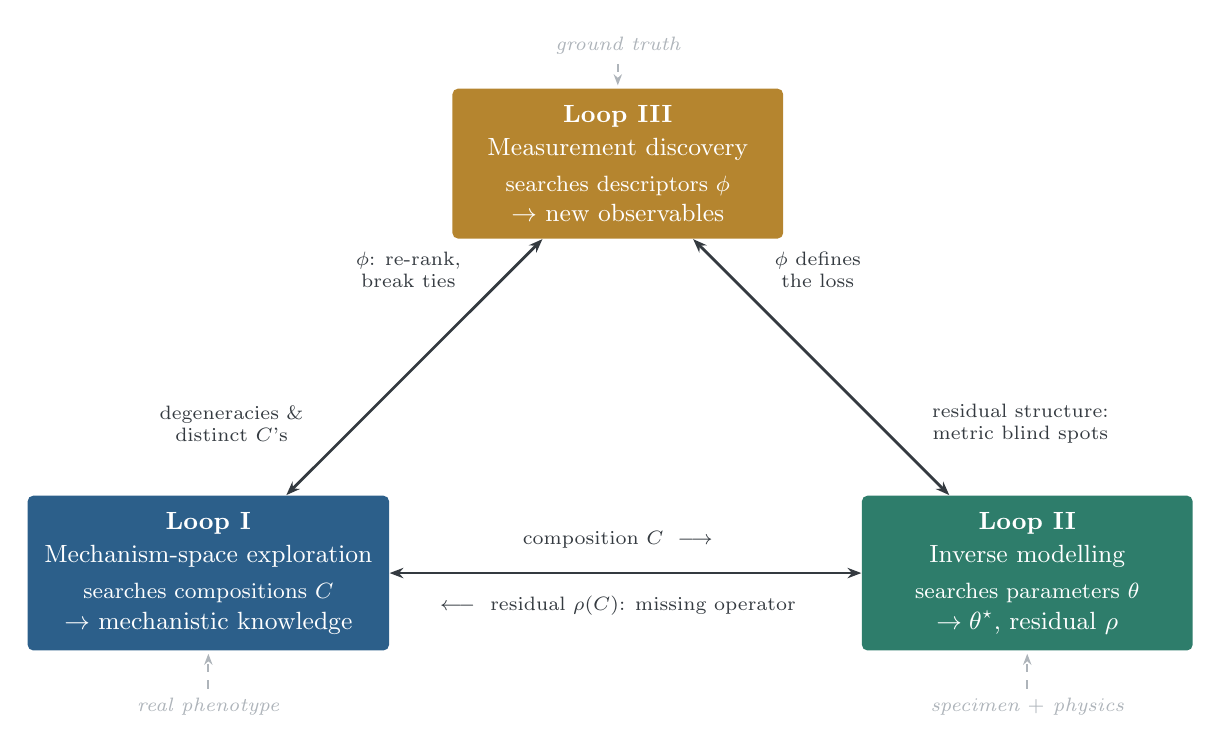
\begin{tikzpicture}[
  >=Stealth,
  box/.style={rounded corners=2pt, align=center, text=white, inner sep=6pt,
              minimum width=4.2cm, minimum height=1.55cm, font=\small},
  edge/.style={{Stealth[length=5pt]}-{Stealth[length=5pt]}, line width=1pt, draw=edgc},
  sig/.style={font=\scriptsize, text=edgc, align=center, inner sep=1pt},
  anch/.style={-{Stealth[length=4pt]}, dashed, line width=0.7pt, draw=anc, shorten >=1pt},
  ancl/.style={font=\scriptsize\itshape, text=anc}]
\node[box, fill=loopone]   (I)   at (-5.2,0) {\textbf{Loop~I}\\[1pt]Mechanism-space exploration\\[2pt]\footnotesize searches compositions $C$\\ $\to$ mechanistic knowledge};
\node[box, fill=looptwo]   (II)  at ( 5.2,0) {\textbf{Loop~II}\\[1pt]Inverse modelling\\[2pt]\footnotesize searches parameters $\theta$\\ $\to \theta^\star$, residual $\rho$};
\node[box, fill=loopthree] (III) at ( 0,5.2) {\textbf{Loop~III}\\[1pt]Measurement discovery\\[2pt]\footnotesize searches descriptors $\phi$\\ $\to$ new observables};
\draw[edge] (I) -- (II);
\draw[edge] (I) -- (III);
\draw[edge] (II) -- (III);
\node[sig] at (0, 0.42) {composition $C\ \longrightarrow$};
\node[sig] at (0,-0.42) {$\longleftarrow\ $ residual $\rho(C)$: missing operator};
\node[sig, anchor=east] at (-3.95,1.9) {degeneracies \&\\ distinct $C$'s};
\node[sig, anchor=east] at (-1.95,3.85) {$\phi$: re-rank,\\ break ties};
\node[sig, anchor=west] at ( 3.95,1.9) {residual structure:\\ metric blind spots};
\node[sig, anchor=west] at ( 1.95,3.85) {$\phi$ defines\\ the loss};
\node[ancl] (gt) at (0,6.7)     {ground truth};
\node[ancl] (rp) at (-5.2,-1.7) {real phenotype};
\node[ancl] (sp) at ( 5.2,-1.7) {specimen $+$ physics};
\draw[anch] (gt) -- (III);
\draw[anch] (rp) -- (I);
\draw[anch] (sp) -- (II);
\end{tikzpicture}
\end{center}
{\small\emph{Three coupled loops over the scientific state $(C,\theta,\phi)$. Each loop searches one space (compositions / parameters / descriptors). Solid edges are two-way signals between loops; dashed edges are the one-way anchoring of each loop to reality that keeps the circle virtuous rather than vicious. Every run is preserved in a shared RunRecord archive, from which the knowledge ledger is distilled.}}

Each edge is two-way. Loop~I hands Loop~II a trusted composition $C$; Loop~II returns the \emph{irreducible} residual $\rho(C)$, which, when systematic, names a \emph{missing operator} rather than a worse parameter---the safeguard the fused loop lacked. Loop~III's descriptor $\phi$ \emph{is} Loop~II's loss, so a sharper metric reshapes the fit, while Loop~II's residual \emph{structure} exposes what $\phi$ cannot yet see. Loop~III's descriptors tighten the emergence test $\mathcal{E}(C)$ and break Loop~I's degeneracies; those degeneracies---compositions the current metric cannot separate---are exactly what Loop~III must learn to tell apart. That same bidirectionality is how a virtuous circle can turn vicious: with no external reference the three loops can agree with one another while drifting from reality. The cure is that each loop is pinned to a fixed point \emph{outside} the triangle---Loop~I to the real phenotype regime, Loop~II to the specimen and its gradients, Loop~III to the ground-truth annotations. The edges are two-way \emph{between} loops; the anchoring is one-way \emph{from reality into} each. Formally the three are block-coordinate ascent on one objective over $(C,\theta,\phi)$, converging to a self-consistent fixed point precisely because the data and ground-truth terms are present; drop them and the joint problem has the trivial degenerate optimum of a metric that calls everything perfect.

\textbf{The bootstrap ladder.} Three equally-active loops would front-load complexity before evidence. The circle instead starts as a ladder, with \emph{only one loop exploratory at a time and the other two frozen as anchors}. Freeze a trusted coarse metric; run Loop~I until one composition robustly enters the real regime across seeds and a parameter basin---and, typically, until several do that the coarse metric cannot tell apart. That degeneracy (or, when a model is already trusted, a structured Loop~II residual) justifies the first revision of the metric; the new measurement then reopens Loop~I wherever it changes the conclusion. The differentiable fit is earned last, never first. A change is promoted only when it \emph{solves a named failure without breaking a previously-established anchor}---a new metric must still agree with ground truth and preserve prior Established verdicts. Versioning ($C$ by structural hash, $\phi$ by metric version) is what makes the coupling converge rather than oscillate.

\section*{Loop I explores primitives; it does not select mechanisms}

The decisive design choice is how Loop~I is parameterised. A search whose branches are named mechanisms---\code{focal\_ecm}, \code{turing}, \code{adhesion}---\emph{selects} the mechanism a priori, the very thing to avoid. The search ranges instead over \emph{primitive} operators (growth, reaction--diffusion, surface-tension/adhesion, boundary/ECM, migration, $\dots$) wired into a \emph{typed graph}: an operator may appear more than once, and a reaction--diffusion morphogen may be routed to place clefts, to gate growth, or to drive chemotaxis---different graphs, different mechanisms. Named mechanisms then \emph{emerge} as discovered regions: if reaction--diffusion coupled to growth generates the phenotype, one has \emph{rediscovered} a Turing mechanism from data. Because the space is graph-valued rather than a Boolean vector, it can explode; the search stays interpretable by editing a composition with exactly \emph{one} legal move at a time (add, remove, or rewire a single operator), stage-gated so each step exposes only a few edits---never an enumeration of the whole space.

Loop~I requires an exploration strategy over that edit tree; any efficient one---random search, Bayesian optimization, evolution, upper-confidence-bound (UCB) search, Monte-Carlo tree search---could be substituted, and a learned surrogate that accelerates it is likewise interchangeable. The contribution is not the search algorithm. It is the separation of forward-model discovery from inverse modelling, and the discipline that every simulation becomes a RunRecord.

\section*{Measurement discovery has its own trap}

Just as fitting parameters to an incomplete model finds a compensating artifact, \emph{fitting a metric to separate two simulation sets} finds a spurious separator---the same disease one level up. Loop~III therefore cannot maximise separation alone. A descriptor is admissible only if it simultaneously agrees with trusted ground truth where it exists (the annotated bud/branch/tube counts), separates compositions Loop~I found phenotypically distinct, and is invariant to nuisance (seed, sampling, resolution). Ground truth is the fixed point that keeps the mechanism and metric loops from co-hallucinating, and it sets the bootstrapping order: the metric is seeded from ground truth first, Loop~I then uses it to define emergence, and Loop~I's residuals and degeneracies drive measurement discovery thereafter.

\section*{The gland case study, in five stages}

\begin{center}
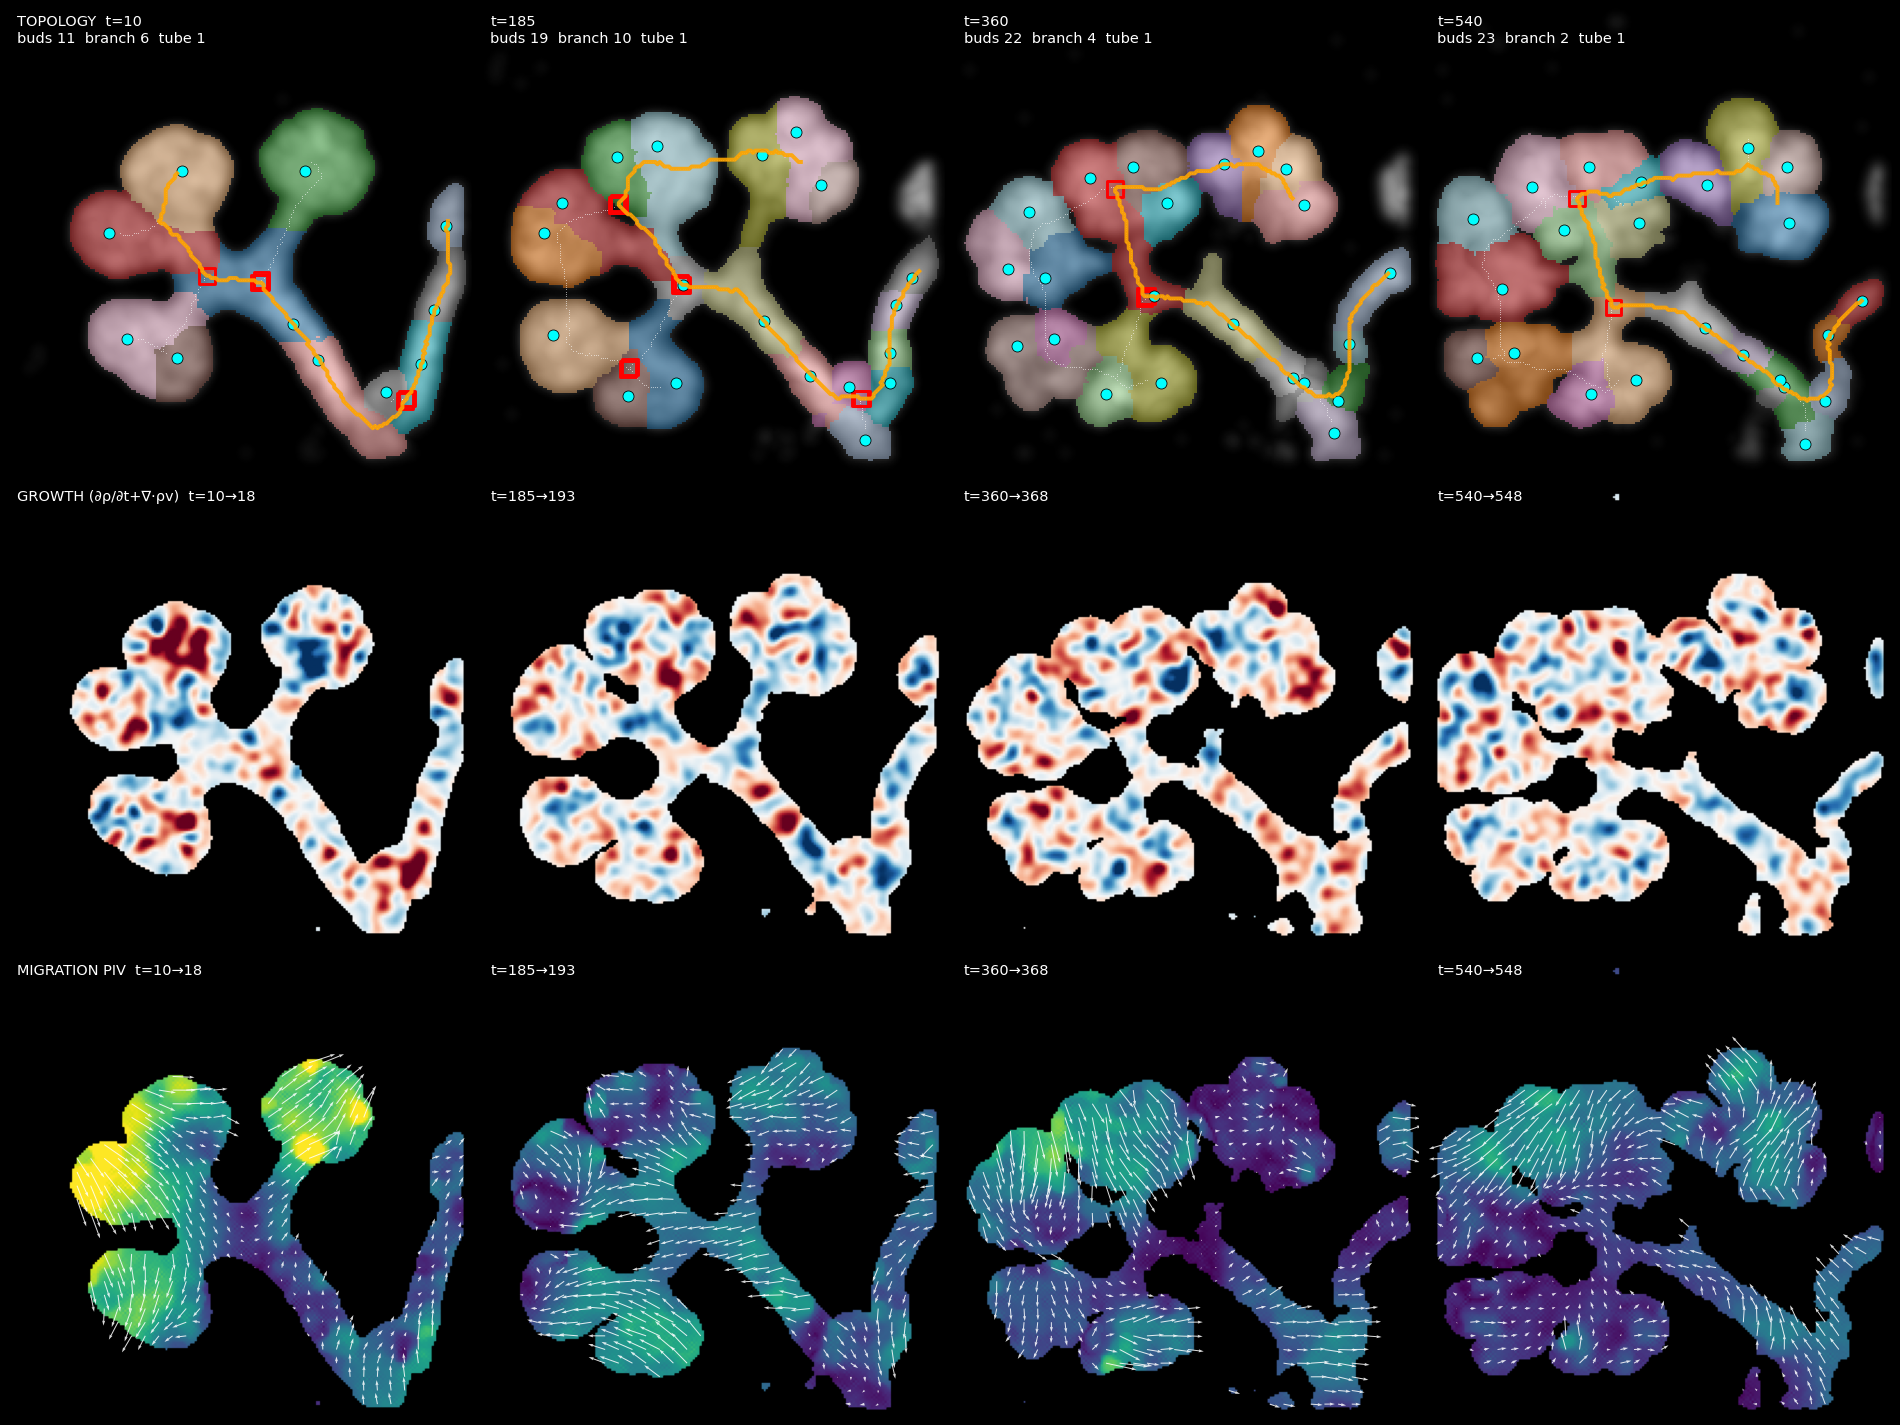
\includegraphics[width=\linewidth]{gland_real_data.png}
\end{center}
{\small\emph{Real embryonic salivary gland (nuclei), four timepoints left to right. Top: topology---a dense, fully-connected epithelium subdivided into lobules by clefts (skeleton $=$ ducts, circles $=$ buds, squares $=$ branch points), one connected mass throughout while lobule count grows. Middle: local growth field. Bottom: collective-migration (particle image velocimetry). These are the observables Loop~III must render reliable and discriminating, and the phenotype Loop~I must make emerge---not a curve to fit.}}

\textbf{Stage~I --- Sparse agents fail.} As the precondition established, a substrate of $\sim\!600$ self-propelled cells fragments---$0/28$ apparent winners survive the corrected readout. \emph{Conclusion: the substrate is insufficient, an expressiveness failure rather than a fitting failure.}

\textbf{Stage~II --- A dense phase field.} We adopt a dense scalar field $u(x,t)\in[0,1]$ (reserving $\phi$ for the descriptor), connected by construction, as the substrate backend; benchmark compositions of primitive operators reproduce, to numerical identity (max deviation $0$), the trajectories of the four hand-built hypotheses---focal ECM, reaction--diffusion, differential adhesion, and confined-growth buckling. \emph{Conclusion: the substrate is now expressive; the operator search can run.}

\textbf{Stage~III --- Mechanism-space exploration.} From a bare seed, one-edit stage-gated exploration runs each composition across a seed and parameter basin; every run is archived as an immutable RunRecord. A first composition---growth with surface tension and a curvature-driven cleft (focal ECM)---robustly enters the real regime (ladder rung~1). The ledger records genuine \emph{structural limitations}: no growth cannot develop, no surface tension fragments, no cleft grows into a blob but cannot subdivide. But under the frozen coarse metric several compositions stay in-regime and none is shown necessary. \emph{Conclusion: two or more plausible forward models, which the current metric cannot separate.}

\textbf{Stage~IV --- Measurement discovery.} The named failure is precise: the initial condition is the real, already-branched $t\!=\!0$ gland, so the topology readout saturates and cannot measure developmental subdivision. A search over an observable bank promotes a subdivision measurement (a lobule-count / perimeter-complexity descriptor) that passes the triple criterion---it agrees with ground truth (subdivision increases from the first to the last imaged frame), separates focal ECM from the reaction--diffusion composition (both discovered by Loop~I---the latter by adding a reaction--diffusion operator and routing it to the cleft source), and is seed-invariant---and re-scores the archived RunRecords by appending a versioned analysis, \emph{without re-simulating}. Re-opening Loop~I's necessity tests under the new metric then closes the circle: the cleft and growth operators, which the coarse metric could not distinguish from decoration, now read as \emph{necessary}, the substrate-only composition is reclassified from ``in regime'' to the structural limitation ``grows but cannot subdivide,'' and focal ECM meets the Established criteria---necessary, sufficient, and robust---for the first time, on this substrate and under the new measurement. \emph{Conclusion: a new measurement changed the mechanism conclusion---the virtuous circle, not loss tuning.}

\textbf{Stage~V --- Differentiable fitting.} Given a trusted composition, a differentiable rollout drives the residual on a synthetic recoverable case from $\sim\!10^{-2}$ to $\sim\!10^{-9}$, recovering the identifiable parameters (surface tension, growth) exactly while exposing a degeneracy between the two cleft-strength parameters---themselves unidentifiable from the final morphology, the kind of structured finding inverse modelling is meant to surface. Fitting a real specimen and reading its irreducible residual as a missing operator is the next rung. \emph{Conclusion: inverse modelling is earned last, never first.}

\section*{Principle}

Inverse modelling assumes the correct model exists and asks for its parameters. Forward-model discovery asks which model should exist at all, and answers it before any parameter is fit. Measurement discovery asks how we should even judge the answer. Separating the three is the contribution: mechanism-space exploration (Loop~I) yields mechanistic knowledge of which operator compositions \emph{generate} the phenotype; inverse modelling (Loop~II) yields the parameters of an earned composition; measurement discovery (Loop~III) yields the observables that can \emph{reliably tell mechanisms apart}. The cardiomyocyte project could fuse discovery and fitting because its mechanism space was effectively a point; salivary gland branching, whose mechanism space is a volume, forces them apart.

What began as a language for biological simulation is becoming an \emph{operating system for computational scientific discovery}: discover the model $\to$ estimate its parameters $\to$ discover how to measure it, with every simulation preserved as evidence and knowledge distilled from it. The particular tools---UCB, surrogates, Adam, phase fields, material-point methods---will change; the three-loop workflow, and the rule that simulation yields records and only records yield knowledge, is what should remain stable across biological domains.

\end{document}
